На рисунке() представлена схема программируемой логики.\par 
\begin{figure}[ht]
    \centering
    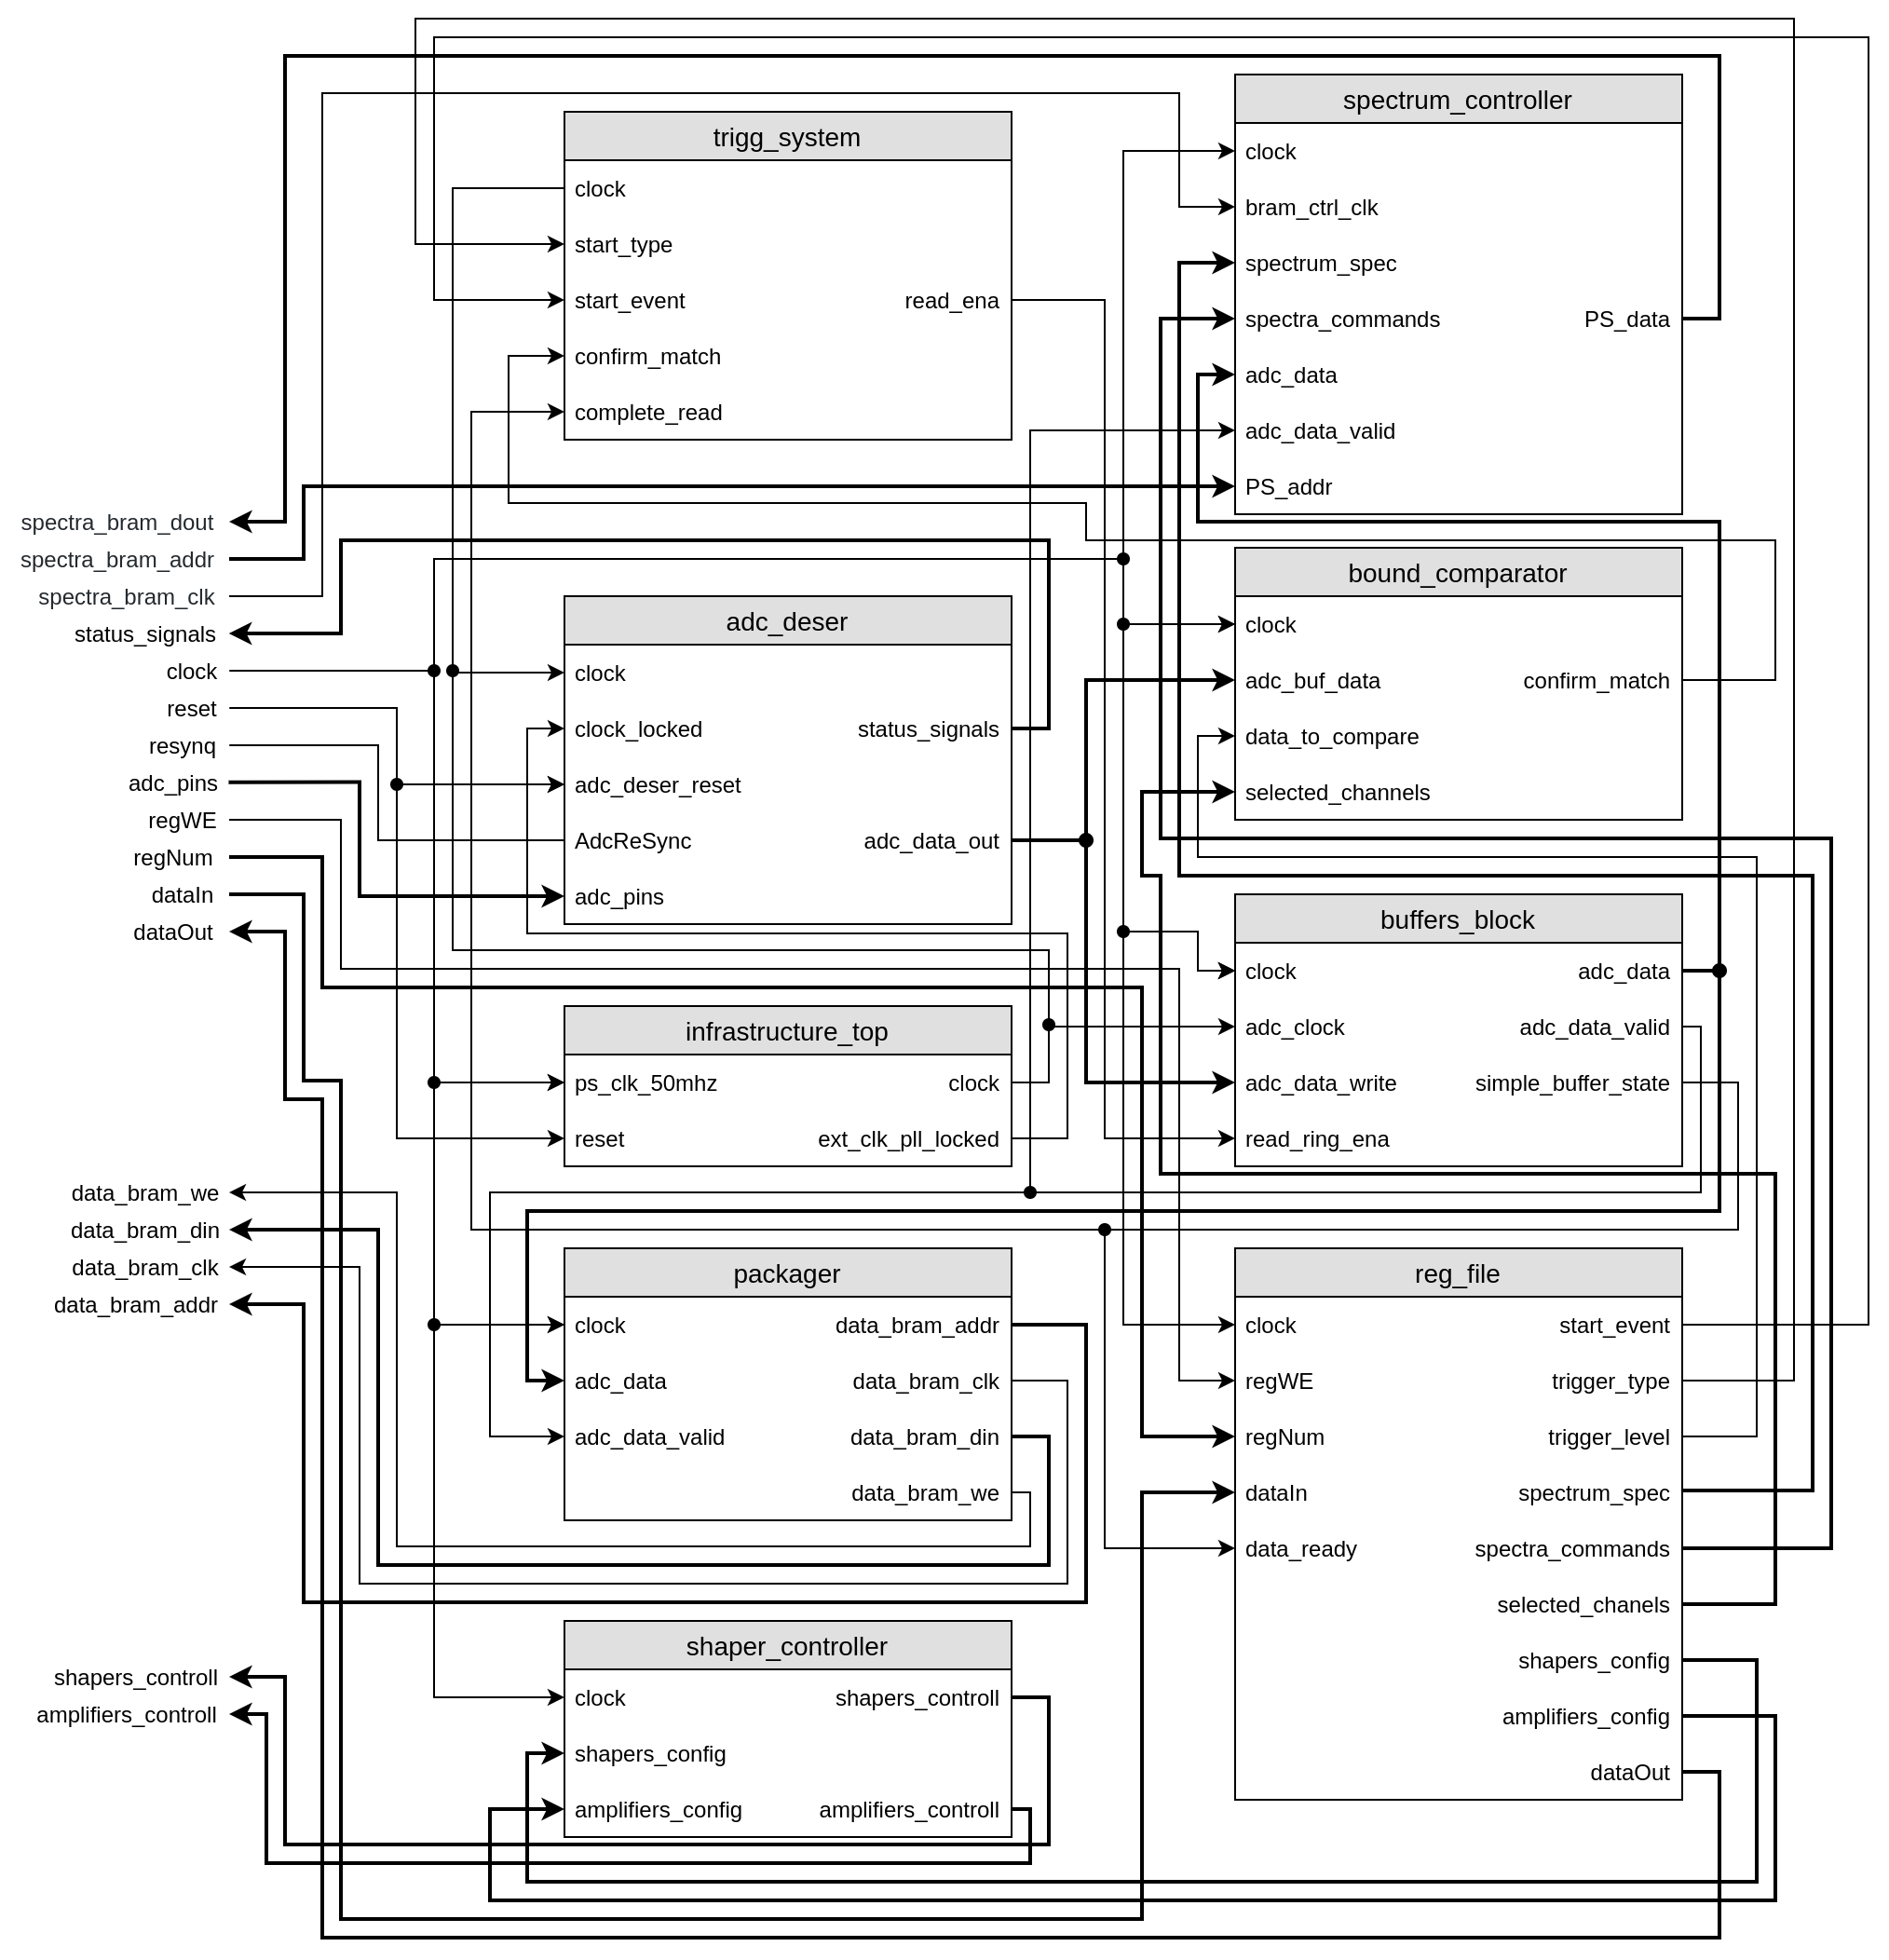
\includegraphics[width=1\linewidth]{PL_top.png}
    \caption{Блок-схема установки}
    \label{fig:mpr}
\end{figure}
Программируемая логика состоит из 9 блоков, краткое описание который представлено в таблице()\par
\begin{table}[h!]
    \caption{Блоки программируемой логики}
   % \begin{tabular}{|>{\centering\arraybackslash}p{0.45\textwidth}|>{\centering\arraybackslash}p{0.45\textwidth}|}
    \begin{tabular}{|p{0.45\textwidth}|p{0.5\textwidth}|}
        \hline
        Наименование блока & Описание \\
        \hline
        adc\_deser & Конвертирует упакованные последовательно данные АЦП в численные значения \\
        \hline
        infrastructure\_top & Обеспечивает тактовую частоту для некоторых модулей \\
        \hline
        packager & Упаковывает данные и передаёт их в процессорную систему \\
        \hline
        shaper\_controller & Осуществляет управление формирователями сигналов \\
        \hline
        spectrum\_creator & Производит обработку данных для набора статистики \\
        \hline
        bound\_comparator & Выполняет сравнение входящих данных с заданными порогами \\
        \hline
        buffers\_block & Буферизует входные данные \\
        \hline
        reg\_file & Реализует блок виртуальных регистров \\
        \hline
        trigg\_system & Генерирует сигнал для сохранения данных \\
        \hline
    \end{tabular}
\end{table}
\textbf{Десериализатор adc\_deser}\par
Одним из основных элементов стенда является АЦП AD-9253. Данный преобразователь работает на 125 МГц параллельно в 4-х каналах. Данные с разрешением 14 бит передаются по протоколу LVDS. Данный стандарт предполагает передачу информации в последовательно-упакованном виде по 2 каналам на каждый вход. На рисунке() представлена временная диаграмма работы АЦП.\par
\begin{figure}[ht]
    \centering
    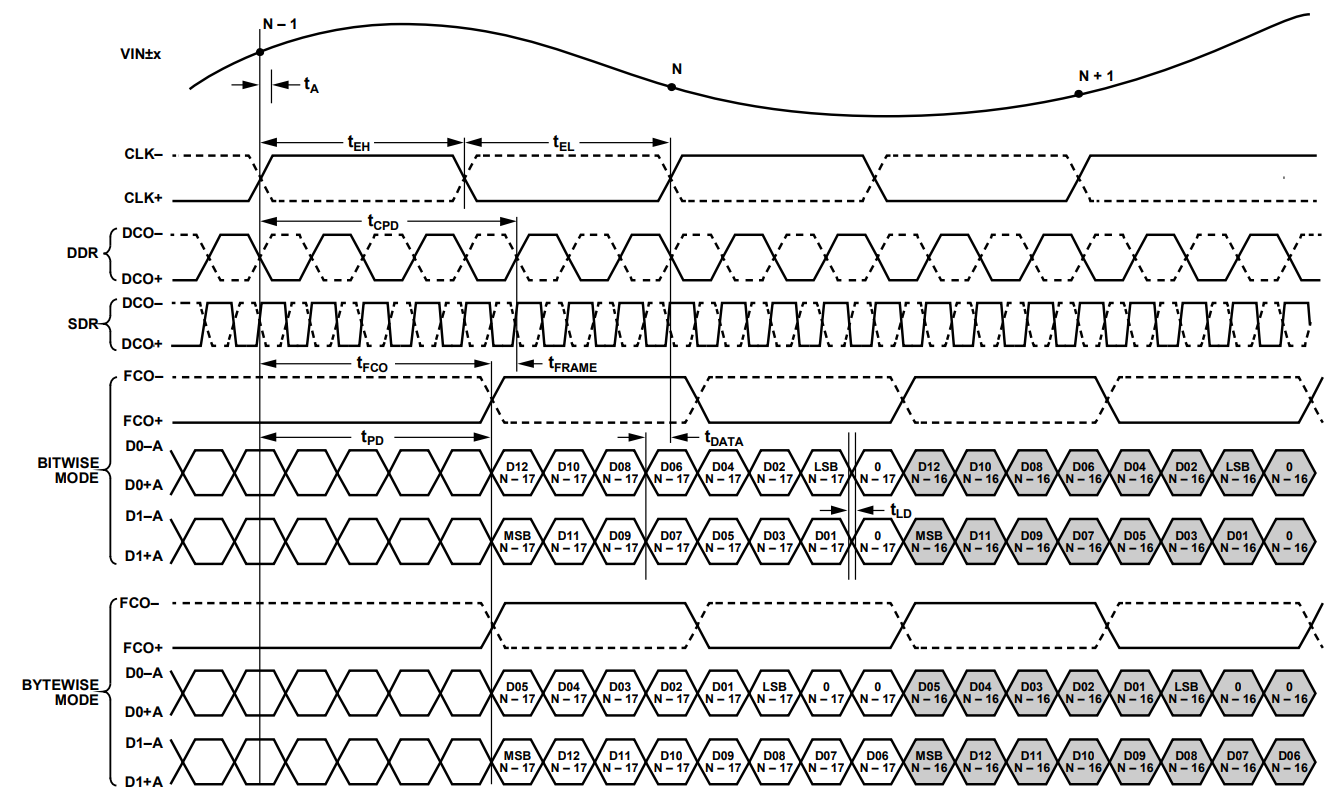
\includegraphics[width=1\linewidth]{ADC_time_diagram.png}
    \caption{Временная диаграмма работы АЦП}
    \label{fig:mpr}
\end{figure}
